\section{Inheritance}

The inheritance can be used as a way to define new classes 
based in more general classes that have been 
defined previously, acquiring their characteristics.  
If a class \emph{CurrentTransformer} directly 
inherits from class \emph{Transformer} we say that 
\emph{Transformer} is the parent 
of \emph{CurrentTransformer} and 
\emph{CurrentTransformer} is the 
child of \emph{Transformer} \cite{Snyder:1986}. 
The UML representation is given in 
Figure \ref{fig:inheritance-fig}.



\begin{figure}
  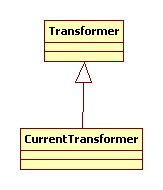
\includegraphics[width=0.3\textwidth]{chapters/ch-oop/figures/inheritance}
  \caption{
  		Inheritance: \emph{Transformer} is the parent 
		of \emph{CurrentTransformer} and 
		\emph{CurrentTransformer} is the 
		child of \emph{Transformer}
		}
  \label{fig:inheritance-fig}
\end{figure}

